\text{FIGURE 2. Another 5-round differential path with probability of $2^{-52}$}

\renewcommand{\arraystretch}{1.5} % Adjust the row height
\setlength{\tabcolsep}{0pt} % Remove extra padding between columns
\begin{center}
    \resizebox{\textwidth}{!}{%
        \(

        \begin{array}{|p{0.5cm}|p{0.5cm}|p{0.5cm}|p{0.5cm}|}
            \hline
            \alpha &  &       & \\ \hline
                   &  &       & \\ \hline
                   &  & \beta & \\ \hline
                   &  &       & \\ \hline
        \end{array}
        \hspace{2pt} % Decrease space here
        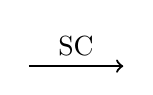
\begin{tikzpicture}[baseline={(current bounding box.center)}, scale=0.4]
            % Arrow from first grid to second grid
            \draw[->, thick] (0, 0) -- (3, 0)
            node[midway, above] {SC};
        \end{tikzpicture}
        \hspace{2pt} % Decrease space here

        \begin{array}{|p{0.5cm}|p{0.5cm}|p{0.5cm}|p{0.5cm}|}
            \hline
            2 &  &   & \\ \hline
              &  &   & \\ \hline
              &  & 2 & \\ \hline
              &  &   & \\ \hline
        \end{array}
        \hspace{2pt} % Decrease space here
        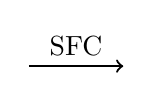
\begin{tikzpicture}[baseline={(current bounding box.center)}, scale=0.4]
            % Arrow from second grid to third grid
            \draw[->, thick] (0, 0) -- (3, 0)
            node[midway, above] {SFC};
        \end{tikzpicture}
        \hspace{2pt} % Decrease space here

        \begin{array}{|p{0.5cm}|p{0.5cm}|p{0.5cm}|p{0.5cm}|}
            \hline
            2 &  &  & \\ \hline
            2 &  &  & \\ \hline
              &  &  & \\ \hline
              &  &  & \\ \hline
        \end{array}
        \hspace{2pt} % Decrease space here
        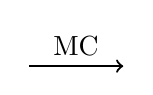
\begin{tikzpicture}[baseline={(current bounding box.center)}, scale=0.4]
            % Arrow from third grid to fourth grid
            \draw[->, thick] (0, 0) -- (3, 0)
            node[midway, above] {MC};
        \end{tikzpicture}
        \hspace{2pt} % Decrease space here
        \begin{array}{|p{0.5cm}|p{0.5cm}|p{0.5cm}|p{0.5cm}|}
            \hline
            2 &  &  & \\ \hline
            2 &  &  & \\ \hline
              &  &  & \\ \hline
              &  &  & \\ \hline
        \end{array}
        \)
        \hspace{2pt} % Decrease space here

        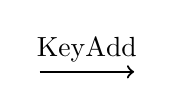
\begin{tikzpicture}[baseline={(current bounding box.center)}, scale=0.4]
            % Arrow from third grid to fourth grid
            \draw[->, thick] (0, 0) -- (3, 0)
            node[midway, above] {KeyAdd};
        \end{tikzpicture}

    }
\end{center}
\begin{center}
    \resizebox{\textwidth}{!}{%
        \(
        \begin{array}{|p{0.5cm}|p{0.5cm}|p{0.5cm}|p{0.5cm}|}
            \hline
            2 &  &  & \\ \hline
            2 &  &  & \\ \hline
              &  &  & \\ \hline
              &  &  & \\ \hline
        \end{array}
        \hspace{2pt} % Decrease space here
        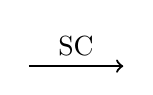
\begin{tikzpicture}[baseline={(current bounding box.center)}, scale=0.4]
            % Arrow from first grid to second grid
            \draw[->, thick] (0, 0) -- (3, 0)
            node[midway, above] {SC};
        \end{tikzpicture}
        \hspace{2pt} % Decrease space here
        \begin{array}{|p{0.5cm}|p{0.5cm}|p{0.5cm}|p{0.5cm}|}
            \hline
            4 &  &  & \\ \hline
            1 &  &  & \\ \hline
              &  &  & \\ \hline
              &  &  & \\ \hline
        \end{array}
        \hspace{2pt} % Decrease space here
        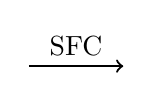
\begin{tikzpicture}[baseline={(current bounding box.center)}, scale=0.4]
            % Arrow from second grid to third grid
            \draw[->, thick] (0, 0) -- (3, 0)
            node[midway, above] {SFC};
        \end{tikzpicture}
        \hspace{2pt} % Decrease space here
        \begin{array}{|p{0.5cm}|p{0.5cm}|p{0.5cm}|p{0.5cm}|}
            \hline
            4 &   &  & \\ \hline
              &   &  & \\ \hline
              &   &  & \\ \hline
              & 1 &  & \\ \hline
        \end{array}
        \hspace{2pt} % Decrease space here
        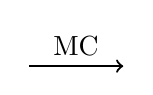
\begin{tikzpicture}[baseline={(current bounding box.center)}, scale=0.4]
            % Arrow from third grid to fourth grid
            \draw[->, thick] (0, 0) -- (3, 0)
            node[midway, above] {MC};
        \end{tikzpicture}
        \hspace{2pt} % Decrease space here
        \begin{array}{|p{0.5cm}|p{0.5cm}|p{0.5cm}|p{0.5cm}|}
            \hline
              & 1 &  & \\ \hline
            4 & 1 &  & \\ \hline
            4 & 1 &  & \\ \hline
            4 &   &  & \\ \hline
        \end{array}
        \)
        \hspace{2pt} % Decrease space here
        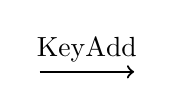
\begin{tikzpicture}[baseline={(current bounding box.center)}, scale=0.4]
            % Arrow from third grid to fourth grid
            \draw[->, thick] (0, 0) -- (3, 0)
            node[midway, above] {KeyAdd};
        \end{tikzpicture}

    }
\end{center}
\begin{center}
    \resizebox{\textwidth}{!}{%
        \(
        \begin{array}{|p{0.5cm}|p{0.5cm}|p{0.5cm}|p{0.5cm}|}
            \hline
              & 1 &  & \\ \hline
            4 & 1 &  & \\ \hline
            4 & 1 &  & \\ \hline
            4 &   &  & \\ \hline
        \end{array}
        \hspace{2pt} % Decrease space here
        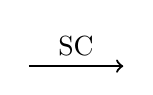
\begin{tikzpicture}[baseline={(current bounding box.center)}, scale=0.4]
            % Arrow from first grid to second grid
            \draw[->, thick] (0, 0) -- (3, 0)
            node[midway, above] {SC};
        \end{tikzpicture}
        \hspace{2pt} % Decrease space here
        \begin{array}{|p{0.5cm}|p{0.5cm}|p{0.5cm}|p{0.5cm}|}
            \hline
              & 2 &  & \\ \hline
            2 & 2 &  & \\ \hline
            2 & 2 &  & \\ \hline
            2 &   &  & \\ \hline
        \end{array}
        \hspace{2pt} % Decrease space here
        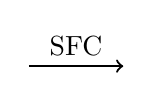
\begin{tikzpicture}[baseline={(current bounding box.center)}, scale=0.4]
            % Arrow from second grid to third grid
            \draw[->, thick] (0, 0) -- (3, 0)
            node[midway, above] {SFC};
        \end{tikzpicture}
        \hspace{2pt} % Decrease space here
        \begin{array}{|p{0.5cm}|p{0.5cm}|p{0.5cm}|p{0.5cm}|}
            \hline
              &   &   &   \\ \hline
              & 2 & 2 &   \\ \hline
            2 &   &   & 2 \\ \hline
              & 2 & 2 &   \\ \hline
        \end{array}
        \hspace{2pt} % Decrease space here
        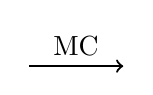
\begin{tikzpicture}[baseline={(current bounding box.center)}, scale=0.4]
            % Arrow from third grid to fourth grid
            \draw[->, thick] (0, 0) -- (3, 0)
            node[midway, above] {MC};
        \end{tikzpicture}
        \hspace{2pt} % Decrease space here
        \begin{array}{|p{0.5cm}|p{0.5cm}|p{0.5cm}|p{0.5cm}|}
            \hline
            2 &   &   & 2 \\ \hline
            2 & 2 & 2 & 2 \\ \hline
              &   &   &   \\ \hline
            2 & 2 & 2 & 2 \\ \hline
        \end{array}
        \)
        \hspace{2pt} % Decrease space here
        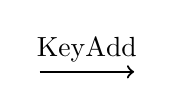
\begin{tikzpicture}[baseline={(current bounding box.center)}, scale=0.4]
            % Arrow from third grid to fourth grid
            \draw[->, thick] (0, 0) -- (3, 0)
            node[midway, above] {KeyAdd};
        \end{tikzpicture}

    }
\end{center}
\begin{center}
    \resizebox{\textwidth}{!}{%
        \(
        \begin{array}{|p{0.5cm}|p{0.5cm}|p{0.5cm}|p{0.5cm}|}
            \hline
            2 &   &   & 2 \\ \hline
            2 & 2 & 2 & 2 \\ \hline
              &   &   &   \\ \hline
            2 & 2 & 2 & 2 \\ \hline
        \end{array}
        \hspace{2pt} % Decrease space here
        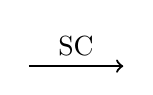
\begin{tikzpicture}[baseline={(current bounding box.center)}, scale=0.4]
            % Arrow from first grid to second grid
            \draw[->, thick] (0, 0) -- (3, 0)
            node[midway, above] {SC};
        \end{tikzpicture}
        \hspace{2pt} % Decrease space here
        \begin{array}{|p{0.5cm}|p{0.5cm}|p{0.5cm}|p{0.5cm}|}
            \hline
            4 &   &   & 1 \\ \hline
            1 & 4 & 1 & 1 \\ \hline
              &   &   &   \\ \hline
            1 & 1 & 1 & 4 \\ \hline
        \end{array}
        \hspace{2pt} % Decrease space here
        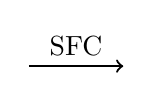
\begin{tikzpicture}[baseline={(current bounding box.center)}, scale=0.4]
            % Arrow from second grid to third grid
            \draw[->, thick] (0, 0) -- (3, 0)
            node[midway, above] {SFC};
        \end{tikzpicture}
        \hspace{2pt} % Decrease space here
        \begin{array}{|p{0.5cm}|p{0.5cm}|p{0.5cm}|p{0.5cm}|}
            \hline
            4 &   & 1 & 1 \\ \hline
              &   & 1 & 1 \\ \hline
            4 & 1 & 1 &   \\ \hline
            4 & 1 &   &   \\ \hline
        \end{array}
        \hspace{2pt} % Decrease space here
        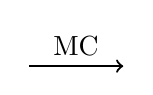
\begin{tikzpicture}[baseline={(current bounding box.center)}, scale=0.4]
            % Arrow from third grid to fourth grid
            \draw[->, thick] (0, 0) -- (3, 0)
            node[midway, above] {MC};
        \end{tikzpicture}
        \hspace{2pt} % Decrease space here
        \begin{array}{|p{0.5cm}|p{0.5cm}|p{0.5cm}|p{0.5cm}|}
            \hline
              &   &   & 1 \\ \hline
            4 &   &   & 1 \\ \hline
              & 1 &   &   \\ \hline
              & 1 & 1 &   \\ \hline
        \end{array}
        \)
        \hspace{2pt} % Decrease space here
        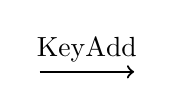
\begin{tikzpicture}[baseline={(current bounding box.center)}, scale=0.4]
            % Arrow from third grid to fourth grid
            \draw[->, thick] (0, 0) -- (3, 0)
            node[midway, above] {KeyAdd};
        \end{tikzpicture}
    }
\end{center}
\begin{center}
    \resizebox{\textwidth}{!}{%
        \(
        \begin{array}{|p{0.5cm}|p{0.5cm}|p{0.5cm}|p{0.5cm}|}
            \hline
              &   &   & 1 \\ \hline
            4 &   &   & 1 \\ \hline
              & 1 &   &   \\ \hline
              & 1 & 1 &   \\ \hline
        \end{array}
        \hspace{2pt} % Decrease space here
        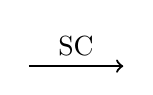
\begin{tikzpicture}[baseline={(current bounding box.center)}, scale=0.4]
            % Arrow from first grid to second grid
            \draw[->, thick] (0, 0) -- (3, 0)
            node[midway, above] {SC};
        \end{tikzpicture}
        \hspace{2pt} % Decrease space here
        \begin{array}{|p{0.5cm}|p{0.5cm}|p{0.5cm}|p{0.5cm}|}
            \hline
              &   &   & 2 \\ \hline
            2 &   &   & 2 \\ \hline
              & 2 &   &   \\ \hline
              & 2 & 2 &   \\ \hline
        \end{array}
        \hspace{2pt} % Decrease space here
        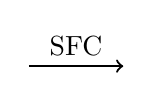
\begin{tikzpicture}[baseline={(current bounding box.center)}, scale=0.4]
            % Arrow from second grid to third grid
            \draw[->, thick] (0, 0) -- (3, 0)
            node[midway, above] {SFC};
        \end{tikzpicture}
        \hspace{2pt} % Decrease space here
        \begin{array}{|p{0.5cm}|p{0.5cm}|p{0.5cm}|p{0.5cm}|}
            \hline
             &   &   & 2 \\ \hline
             &   &   & 2 \\ \hline
             & 2 & 2 &   \\ \hline
             & 2 & 2 &   \\ \hline
        \end{array}
        \hspace{2pt} % Decrease space here
        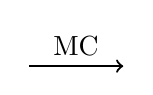
\begin{tikzpicture}[baseline={(current bounding box.center)}, scale=0.4]
            % Arrow from third grid to fourth grid
            \draw[->, thick] (0, 0) -- (3, 0)
            node[midway, above] {MC};
        \end{tikzpicture}
        \hspace{2pt} % Decrease space here
        \begin{array}{|p{0.5cm}|p{0.5cm}|p{0.5cm}|p{0.5cm}|}
            \hline
             &   &   & 2 \\ \hline
             &   &   & 2 \\ \hline
             & 2 & 2 &   \\ \hline
             & 2 & 2 &   \\ \hline
        \end{array}
        \hspace{2pt} % Decrease space here
        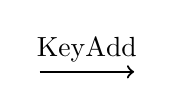
\begin{tikzpicture}[baseline={(current bounding box.center)}, scale=0.4]
            % Arrow from third grid to fourth grid
            \draw[->, thick] (0, 0) -- (3, 0)
            node[midway, above] {KeyAdd};
        \end{tikzpicture}
        \hspace{2pt} % Decrease space here
        \begin{array}{|p{0.5cm}|p{0.5cm}|p{0.5cm}|p{0.5cm}|}
            \hline
             &   &   & 2 \\ \hline
             &   &   & 2 \\ \hline
             & 2 & 2 &   \\ \hline
             & 2 & 2 &   \\ \hline
        \end{array}
        \)
    }
\end{center}